\documentclass[11pt,letterpaper,onecolumn]{article}

\usepackage[utf8]{inputenc}
\usepackage[spanish]{babel}
\usepackage{float}
\usepackage{eurosym}
\usepackage{xcolor}
\usepackage{verbatim}
\usepackage{mwe}
\usepackage{charter}
\usepackage{afterpage}
\usepackage{amsmath}
\usepackage{appendix}
\usepackage{ragged2e}
\usepackage{array}
\usepackage{etoolbox}
\usepackage{fancyhdr}
\usepackage{booktabs}
\usepackage{arydshln}
\usepackage{enumitem}
\usepackage[bottom=2.5cm,top=2.0cm,left=2.0cm,right=2.0cm]{geometry}
\usepackage{graphicx}
\usepackage{indentfirst}
\usepackage{mathtools}
\usepackage{multirow}
\usepackage{pdfpages}

\usepackage{subfiles}
\usepackage[compact]{titlesec}
\usepackage{blindtext}
\usepackage{stfloats}
\usepackage{lipsum} 


\renewcommand{\familydefault}{\rmdefault}

\newcommand\blankpage{
    \null
    \thispagestyle{empty}
    \addtocounter{page}{0}
    \newpage}

\newcolumntype{L}[1]{>{\raggedright\let\newline\\arraybackslash\hspace{0pt}}m{#1}}
\newcolumntype{C}[1]{>{\centering\let\newline\\arraybackslash\hspace{0pt}}m{#1}}
\newcolumntype{R}[1]{>{\raggedleft\let\newline\\arraybackslash\hspace{0pt}}m{#1}}

    \setlist[itemize,1]{label=$\bullet$}
    \setlist[itemize,2]{label=$\circ$}
    \setlist[itemize,3]{label=$-$}
    \setlist{nosep}

\setlength{\columnsep}{30pt}

\titlelabel{\thetitle.\quad}

\pagestyle{fancy}
\fancyhf{}
      
\fancyfoot{}
\fancyfoot[C]{\thepage} % page
\renewcommand{\headrulewidth}{0mm} % headrule width
\renewcommand{\footrulewidth}{0mm} % footrule width

\makeatletter
\patchcmd{\headrule}{\hrule}{\color{black}\hrule}{}{} % headrule
\patchcmd{\footrule}{\hrule}{\color{black}\hrule}{}{} % footrule
\makeatother

\definecolor{blueM}{cmyk}{1.0,0.49,0.0,0.47}

%%%%%%%%%%%%%%%%%%%%%%%%%%%%%%%%%%%%%%%%%%%%%%%%%%%%%%%%%%%%%%%%%%%%%%%%%%%%%%%%%%%%%%%%%%%%%%%%%%%%%%%%%%%%%%%%%%%%%%%%%%%%%%%%%%%%%%%%%%%%%%%%%%%%%%%%%%%%%%%%%%%%%%%%%%%%%%%%%%%%%%%%%%%%%%%%%%%%%%%%%%%%%%
%%%%%%%%%%%%%%%%%%%%%%%%%%%%%%%%%%%%%%%%%%%%%%%%%%%%%%%%%%%%%%%%%%%%%%%%%%%%%%%%%%%%%%%%%%%%%%%%%%%%%%%
\chead[C]{
      \begin{tabular}{m{1.5cm}m{11.5cm}m{2.5cm}}
      
\includegraphics[height=1.5cm]{logo.png}
      &
      \centering
      \fcolorbox{white}{white}{\fbox{\begin{minipage}{11.9cm}
     \centering
     \textcolor{blueM}{ Prácticas Evaluación Financiera}
     \end{minipage}}}
         &
        \centering
         \tiny{ \vspace{3.5mm} Grado en Física \\  %para usar en otras carreras consulte a su coordinador
%%%%%%%%%%%%%%%%%%%%%%%%%%%%%%%%%%%%%%%%%%%%%%%%%%%%%%%%%%%%%%%%%%%%%%%%%%%%%%%%%%%%%%%%%%%%%%%%%
             %elija el que corresponda ejemplo :  Modular : I
%%%%%%%%%%%%%%%%%%%%%%%%%%%%%%%%%%%%%%%%%%%%%%%%%%%%%%%%%%%%%%%%%%%%%%%%%%%%%%%%%%%%%%%%%%%%%%%%%
            Página \thepage \hspace{1pt} de 10
          }\tabularnewline
%          \hline
          \end{tabular}%
    }
    
\begin{document}


\hspace{25pt}
\begin{minipage}{0.8\textwidth}
\begin{center}
	
	\vspace{5mm}

	\Large{\textbf{Asignatura de Proyectos. 3º Física}} %
    \\ 
    \large{\textbf{Martín Romero, Álvaro}. \textcolor{blueM}{f82maroa@uco.es}} % Si solo hay un autor borrar el apartado sin borrar el ultimo }\\ 
   \\ 
    \vspace{3mm}
    \fontsize{0.35cm}{0.5cm}\selectfont \textit{Departamento de Física, UCO, Universidad de Córdoba}
    \vspace{1mm} 
    
    \today % FECHA

\end{center}
\end{minipage}

\small

\vspace{11pt}

\centerline{\rule{0.95\textwidth}{0.4pt}}

\begin{center}
    
    \begin{minipage}{0.9\textwidth}
        % RESUMEN
	    \noindent \textbf{Resumen:} En estas prácticas pondremos en práctica los conocimientos adquiridos en clase sobre los métodos de reconocimiento de rentabilidad de proyectos financieros. Calcularemos variables como la \textbf{TIR}, \textbf{VAN} o el coeficiente \textbf{Q} y demás datos, en vez de a mano como hicimos en clase, en hojas de cálculo.
    
        \vspace{4mm}
        % PALABRAS CLAVE
    
    \end{minipage}
    
\end{center}
\centerline{\rule{0.95\textwidth}{0.4pt}}
\vspace{15pt}
\section{Ejercicio 1}%
\label{sec:Ejercicio 1}
\begin{figure}[h]
	\centering
	\caption{Tabla de valores con los datos que nos dan del proyecto}	
	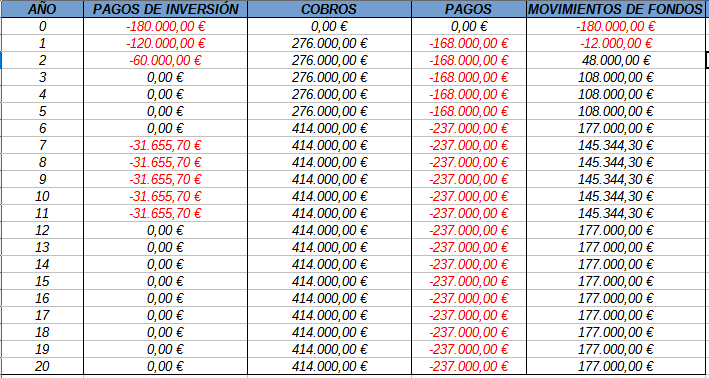
\includegraphics[width=0.8\textwidth]{imagen/ej1_1.PNG}
\end{figure}
La figura ilustra los datos del proyecto que nos da el problema. Se trata de un proyecto de una vida de 20 años con inversión en los 2 primeros años y una reinversión desde los años 7 al 11. El interés de mercado es de un valor del 11\%. El producto se vende a 1.20 € la unidad, con 1000 unidades en un día los primeros 5 años y 1500 ud/día los siguientes años. \\ 
\\
Siguiendo los pasos dados por el protocolo de prácticas, calcularemos las variables \textbf{VAN}, \textbf{Q} y \textbf{TIR}. La figura 2 ilustra los valores de esas variables
\newpage
\hspace{5cm}
\subsection{Apartado a}
\begin{figure}[H]
	\centering
	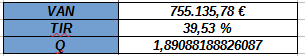
\includegraphics[width=0.3\textwidth]{imagen/ej1_van.PNG}
	\caption{VAN, Q y TIR del proyecto}
	\label{fig:}
\end{figure}
Como podemos observar, el proyecto es rentable puesto que el VAN, por tanto, la Q son positivas. La Q tiene un valor aproximado del $Q=1.89 \%$, esto es, cada euro que invertimos en el proyecto, obtenemos un beneficio de 2,89 €, el euro invertido más 1.89 € obtenido. \\
\\
La TIR muestra el valor de interés que tendría llevar la inversión al banco. Un valor de interés del 39.53\%
\subsection{Apartado b}
Nos piden el precio mínimo que tendría que tener el producto para que la inversión siga siento rentable. Esto se traduce en decir que tenemos que hallar el precio de $p$ para que el VAN sea 0. A partir del valor de VAN 0 consideramos que la inversión ha sido rentable. \\
\\
Para hacer esto en la hoja de datos, llevamos el precio de $p$ hasta que el valor del VAN pase de negativo a postivo. Este valor se halla en 
\[
	\boxed{p_{min}=0.8749 $€$}
.\] 
Esto es, el precio del producto tendría que ser a partir de 0.8749 €
\subsection{Apartado c}
Nos piden calcular el periodo de recuperación. Esto es, ver el año donde la inversión se recupera. Para ello calculamos el VAN año a año, lo vemos en la figura \ref{rec}
\begin{figure}[H]
	\centering
	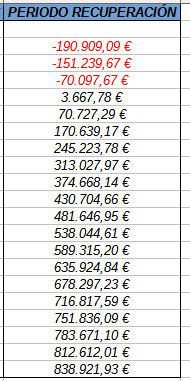
\includegraphics[width=0.23\textwidth]{imagen/ej1_rec.PNG}
	\caption{Cálculo del periodo de recuperación. La casilla que no tiene ningún valor corresponde al año 0, la siguiente al 1 y así sucesivamente hasta el año 20.}
	\label{rec}
\end{figure}
\newpage
\vspace{8cm}
Como vemos, el año donde el VAN comienza a ser positivo es en el año 4. Del año 3 al 4 el proyecto empieza a ser rentable, siendo este periodo de recuperación relativamente corto. Aunque arriesgado debido a la gran inversión inicial y a las pérdidas que suponen los primeros años. Después del año de recuperación, las ganancias son bastante altas, algo que sabíamos inicialmente con el valor del TIR, Q y VAN. \\
\\
Concluimos dando por hecho que se trata de un proyecto rentable en poco tiempo a pesar del riesgo que supone invertir gran cantidad de dinero los primeros años. 
\section{Ejercicio 2}%
\label{sec:Ejercicio 2}

 Tenemos un proyecto de 7 años con un interés al 8\%. Los costes de desarrollo son de 300.000 €. Durante los 3 primeros años, los costes de correcto funcionamiento son de 3.000€/unidad. 
 \subsection{Apartado a}
\begin{itemize}
\item 
	Nos piden hallar el precio mínimo de venta del producto. Esto es, al igual que antes, encontrar el valor del precio del producto para que el VAN pase de negativo a positivo. Hecho esto, mostramos el valor de los movimientos de fondos cada año para calcular el VAN, TIR y Q del proyecto con un valor del precio mínimo de 5.609,30€:
  \begin{figure}[H]
 	\centering
	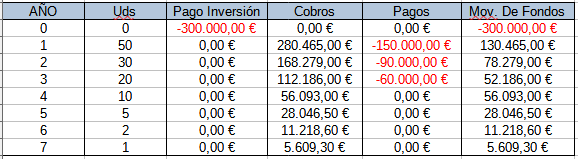
\includegraphics[width=0.8\textwidth]{imagen/ej2a_1.PNG}
	\caption{Datos con los años, unidades de producto y movimiento de fondos cada año}
 	\label{fig:2a1}
 \end{figure}
 Con este valor de precio de producto, obtenemos:
 \begin{figure}[H]
 	\centering
	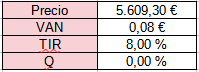
\includegraphics[width=0.23\textwidth]{imagen/ej2a_1_van.PNG}
	\caption{Variables VAN, Q y TIR para el precio mínimo}
 	\label{fig:2}
 \end{figure}
 Como vemos, el valor del VAN es muy cercano a 0, a partir de este valor de precio de producto, el proyecto empieza a ser rentable. La TIR se corresponde al valor del interés debido a que el VAN y por consiguiente la Q son nulas.
 \item Nos piden el valor del precio del producto por unidad para un valor de la TIR del 20\% y del 30\%. Para ello variamos el precio del producto hasta encontrar esos valores de la TIR:
	 \begin{figure}[H]
	 	\centering
		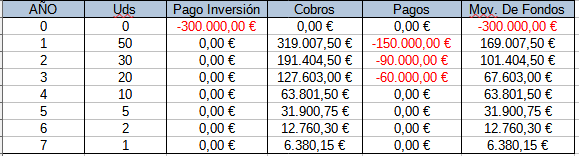
\includegraphics[width=0.8\textwidth]{imagen/ej2a_2.PNG}
	 	\caption{Datos para la TIR de 20\%}
	 	\label{fig:imagen-ej2a_2-PNG}
	 \end{figure}	
	 \begin{figure}[H]
	 	\centering
		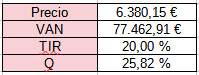
\includegraphics[width=0.23\textwidth]{imagen/ej2a_2_van.PNG}
	 	\caption{Valor del precio para la TIR de 20\%}
	 	\label{fig:imagen-ej2a_2_van-PNG}
	 \end{figure}
	 \begin{figure}[H]
	 	\centering
		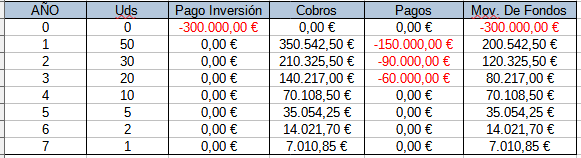
\includegraphics[width=0.8\textwidth]{imagen/ej2a_3.PNG}
	 	\caption{Datos para la TIR de 30\%}
	 	\label{fig:imagen-ej2a_3-PNG}
	 \end{figure}
	 \begin{figure}[H]
	 	\centering
		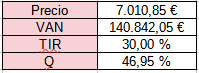
\includegraphics[width=0.23\textwidth]{imagen/ej2a_3_van.PNG}
	 	\caption{Valor del precio del producto para la TIR de 30\%}
	 	\label{fig:imagen-ej2a_3_van-PNG}
	 \end{figure}
\end{itemize}

\subsection{Apartado b}
Nos piden determinar si es interesante la siguiente opción: Con el precio del producto de 6000 €/unidad, los costes de mantenimiento se pueden reducir a 1500 €/unidad si invertimos un valor de 440.000€ en desarrollo (es decir, su primer año). \\
\\
Con los datos dados, cambiamos los valores dados en el apartado anterior, obteniendo la siguiente tabla:
\begin{figure}[H]
	\centering
	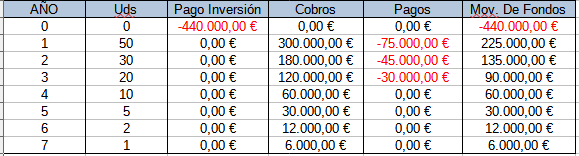
\includegraphics[width=0.8\textwidth]{imagen/ej2b_mod.PNG}
	\caption{Valores de movimiento de fondos para un precio de producto de 6000 €/unidad con un coste de reforma de 1500€/u y un pago de inversión de desarrollo de 440.000€}
	\label{fig:imagen-ej2b_mod-PNG}
\end{figure}	
Calculamos la TIR, la Q y el VAN de esta propuesta del proyecto
\begin{figure}[H]
	\centering
	\includegraphics[width=0.23\textwidth]{imagen/ej2b_mod_VAN.png}
	\caption{VAN, TIR y Q para el proyecto con 6000€/unidad}
	\label{fig:imagen-ej2b_mod_VAN-png}
\end{figure}
Según vemos en la figura 11 parece ser rentable, ya que el VAN tiene un valor positivo, pero para saber si merece la pena aumentar el pago de inversión de desarrollo para disminuir el pago por producto compararemos con la situación inicial con un valor de precio de producto de 6.000€/unidad:
\begin{figure}[H]
	\centering
	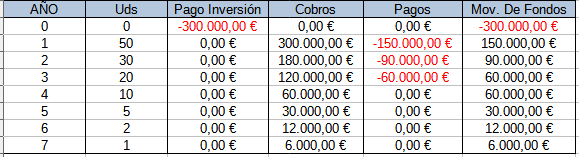
\includegraphics[width=0.8\textwidth]{imagen/ej2b_or.PNG}
	\caption{Tabla de valores para las condiciones iniciales con un valor de precio de producto de 6000€/u}
	\label{fig:imagen-ej2b_or-PNG}
\end{figure}
\begin{figure}[H]
	\centering
	\includegraphics[width=0.23\textwidth]{imagen/ej2b_or_VAN.PNG}
	\caption{VAN, TIR y Q para condiciones iniciales}
	\label{fig:imagen-ej2b_or_VAN-PNG}
\end{figure}
Como vemos, en las condiciones iniciales, el VAN es mayor que el VAN con las condiciones impuestas posteriormente, por tanto, podemos decir que esta opción no es interesante, perderíamos dinero además de introducir una inversión mayor inicial, lo que supone más riesgo inicial.
\subsection{Apartado c}
En este apartado nos piden la cantidad mínima de producto vendido constantemente en los años para que sea rentable el proyecto. Para eso, debemos de ir cambiando la casilla de unidades por valores constantes en los 7 años. Encontramos que el valor que hace que el VAN sea positivo es de 13 unidades por año (el resultado exacto sale 12,.. sin embargo, aproximamos a 13 ya que no tiene sentido hablar de unidades de producto con números no enteros)
\begin{figure}[H]
	\centering
	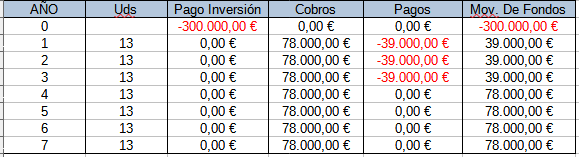
\includegraphics[width=0.8\textwidth]{imagen/ej2c.PNG}
	\caption{Tabla de datos con unidades de 13 por año}
	\label{fig:ej2c-PNG}
\end{figure}
\begin{figure}[H]
	\centering
	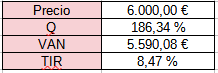
\includegraphics[width=0.23\textwidth]{imagen/ej2c_van.png}
	\caption{VAN, TIR y Q para valores de 13 unidades. Vemos que el VAN no es muy cercano a 0. A un menor valor de unidades, obtendríamos un valor negativo del VAN, así que 13 es el valor que nos piden}
%	\label{figoo}
\end{figure}
\subsection{Apartado d}
Para saber la proporcionalidad de unidades teniendo las condiciones iniciales, multiplicamos la columna de unidades por una constante hasta obtener un valor de Q=150\%
\begin{figure}[H]
	\centering
	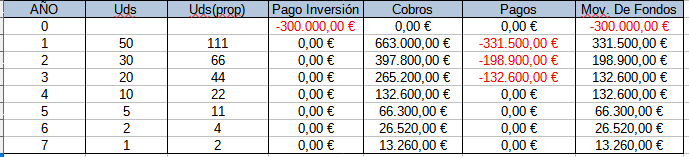
\includegraphics[width=0.8\textwidth]{imagen/ej2d.PNG}
	\caption{Datos para calcular la constante de proporcionalidad. Hemos multiplicado la columna de unidades inicialmente por un valor de 2.21 para que Q sea lo más parecido a 150\%}
	\label{fig:imagen-ej2d-PNG}
\end{figure}
\begin{figure}[H]
	\centering
	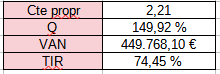
\includegraphics[width=0.23\textwidth]{imagen/ej2d_van.PNG}
	\caption{Vemos que para un valor de constante de proporcionalidad de 2.21, el valor de Q es muy parecido a 150\%, el valor que nos piden.}
	\label{fig:imagen-ej2d_van-PNG}
\end{figure}

\section{Ejercicio 3}%
\label{sec:Ejercicio 3}
El proyecto que vamos a estudiar tiene un tiempo estimado de vida de 12 años con un interés variable: 1-3 años 12\%, 4-5: 10\%, 6-12: 8\%. La inversión consta de 2 inversiones en el año 0 y 1 con una reinversión de anualidad al 10\% durante los años 6,7 y 8:
\begin{figure}[H]
	\centering
	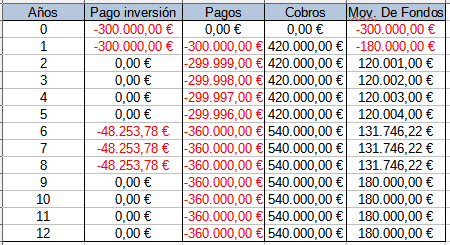
\includegraphics[width=0.8\textwidth]{imagen/ej3a.png}
	\caption{Datos del proyecto}
	\label{fig:imagen-}
\end{figure}
\subsection{Apartado a}
Tenemos que calcular el VAN para diferentes intereses. Para ello calculamos el VAN de los diferentes años cada uno con su interés y lo llevamos al año 0, posteriormente los sumamos, es decir, la ecuación que tenemos que despejar para hallar el VAN es:
\[
	VAN=VAN(0-3)+\frac{VAN(4-5)}{(1+0,12)^3}+ \frac{VAN(6-12)}{(1+0,12)^3(1+0,08)^2}
.\] 
Obtenemos por tanto la siguiente tabla para el VAN y la Q:
\begin{figure}[H]
	\centering
	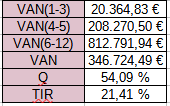
\includegraphics[width=0.23\textwidth]{imagen/ej3a_van.PNG}
	\caption{VAN para los diferentes intereses y el VAN llevado al año 0}
	\label{fig:imagen-ej3a_van-PNG}
\end{figure}
Vemos que el resultado del VAN es positivo, por tanto, también lo es la Q. Esto nos indica que el proyecto es rentable, además podemos observar que el tiempo de recuperación es bastante corto, aunque el pago de inversión es considerablemente elevado. Por último destacar el valor de la Q=54.09\%, esto nos indica que si invertimos un euro en el proyecto, obtendremos el euro invertido más 1,54 euros más. \\
\\
El valor de la TIR es de 21,41\%. Esto es, el valor del interés si queremos obtener el mismo beneficio llevando el dinero de la inversión al banco con ese interés.\\ 
\\
Concluimos diciendo que la inversión en este proyecto es bastante rentable a pesar de las dos inversiones altas de los dos primeros años.
\subsection{Apartado b}
Analizaremos ahora si la inversión sigue siendo rentable si quitando la reinversión, los movimientos de fondo disminuyen en un 10\%. Esto es equivalente a restarle el 10\% a la columna de los movimientos de fondo, esto queda tal que
dig
\begin{figure}[H]
	\centering
	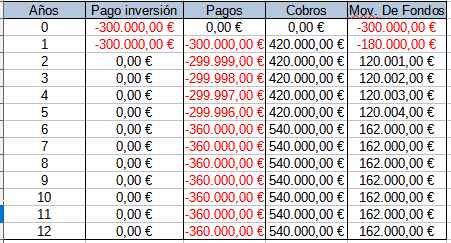
\includegraphics[width=0.8\textwidth]{imagen/ej3b.PNG}
	\caption{Proyecto con movimiento de fondo disminuido el 10\%, quitando la reinversión a partir del año 6}
	\label{fig:imagen-ej3b-PNG}
\end{figure}
Calculamos el VAN tal como hicimos anteriormente:
\begin{figure}[H]
	\centering
	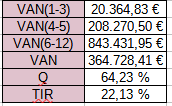
\includegraphics[width=0.23\textwidth]{imagen/ej3b_van.PNG}
	\caption{VAN y Q para las nuevas condiciones impuestas}
	\label{fig:imagen-ej3b_van-PNG}
\end{figure}
Podemos apreciar un aumento considerable de la Q, siendo esta un 10\% más alta. El VAN tiene un valor considerablemente parecido al proyecto con las anteriores condiciones.\\
\\
Con la Q un 10\% más alta, cuando invertimos en el proyecto 1 euro, obtendremos 10 centimos más que con las anteriores condiciones, a parte de que no tendremos los riesgos que supone la reinversión.\\
\\
Concluimos diciendo que esta opción es más rentable que la anterior.
\section{Ejercicio 4}
El proyecto cuenta con una inversión inicial dividida en los años 0 y 1. Después hay una reinversión, la primera anual al 12\% de 150.000€ durante los años 3-6 y una segunda en el año 7 de 300.000€, teniendo un valor residual de la inversión anterior de 30.000€.\\
\\
El tiempo de vida del proyecto es de 15 años, con una inflación del 3\% y un interés variable: año 1-5 del 10\% y 8\% el resto. \\
\\
Los productos tienen un beneficio de 15€/unidad, con una producción anual variable y costes tales que : $Coste=30000+3\cdot p$ siendo p la producción anual
\begin{figure}[H]
	\centering
	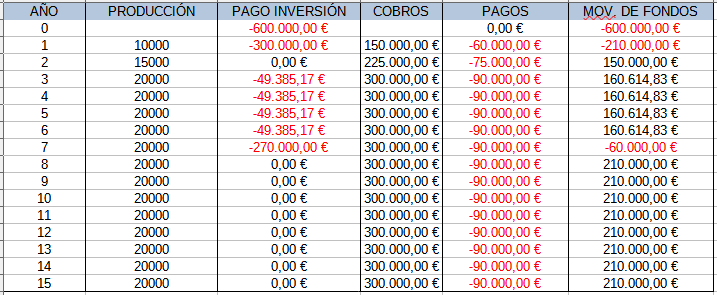
\includegraphics[width=0.8\textwidth]{imagen/ej4a.png}
	\caption{Datos del proyecto}
	\label{fig:ej4a-png}
\end{figure}
\subsection{Apartado a}
Nos piden calcular la rentabilidad según el VAN y la Q.\\
\\
La inflación hace que tengamos que modificar el valor del interés de mercado, restándole el valor de esta inflación para obtener el valor de interés real, siendo por tanto la inflación del 3\%, el interés será del 7\% durante los años 1-5 y 5\% el resto.\\
\\
Calculamos el VAN de la misma forma que hacíamos en el ejercicio anterior, quedando:
\begin{figure}[H]
	\centering
	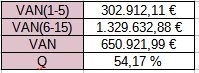
\includegraphics[width=0.23\textwidth]{imagen/ej4a_van.PNG}
	\caption{VAN de diferentes años según el interés y pasado al actual junto con  la Q}
	\label{fig:imagen-ej4a_van-PNG}
\end{figure}
Vemos que el valor del VAN y de la Q son positivos y elevados, por tanto, podemos decir que el proyecto es rentable. Observamos que al tener que hacer pagos de reinversiones el valor del VAN disminuye, aunque el proyecto sigue siendo rentable haciendo estas reinversiones. \\
\\
El valor de la Q=54.17\% nos indica que por cada euro invertido en el proyecto obtenemos el euro invertido más 1.54€.\\
\\
Por tanto, concluimos diciendo que aunque el proyecto tiene un riesgo elevado debido al alto valor de los pagos iniciales y posteriores, el proyecto es rentable. 

\subsection{Apartado b}
Al principio obtenemos una TIR del 12,86\%, pero debemos de sumar el valor de la inflación sobre la TIR. Corregida esta, queda una TIR del 15,86\%; esto es, el valor del interés de mercado con el que obtendríamos beneficio si invertimos el mismo dinero en el banco. 
\subsection{Apartado c}
Para medir la sensibilidad del producto, multiplicamos por una constante a la columna del producto hasta que el VAN sea muy parecido a 0. Obtenido este valor, introducimos la tabla con los datos:
\begin{figure}[H]
	\centering
	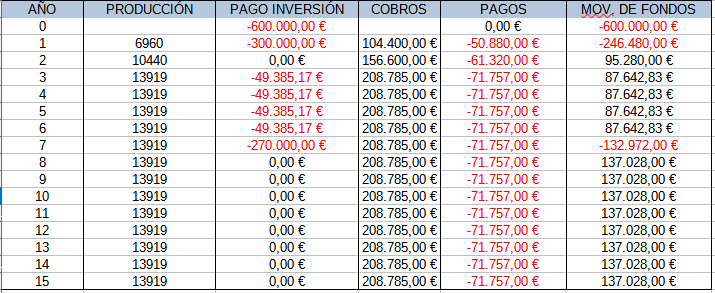
\includegraphics[width=0.8\textwidth]{imagen/ej4c.PNG}
	\caption{Datos de la producción cambiando el valor de la constante para hacer el VAN lo más posible cerca a 0}
	\label{fig:imagen-ej4c-PNG}
\end{figure}
El valor de esta constante es de 0.5 el primer año y 0.75 el año 2.
\begin{figure}[H]
	\centering
	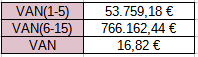
\includegraphics[width=0.23\textwidth]{imagen/ej4c_van.PNG}
	\caption{Valor del VAN, donde vemos que es muy cercano a 0}
	\label{fig:imagen-ej4c_van-PNG}
\end{figure}


\end{document}

